\section{extrasolar: todo}

\begin{wordonframe}{Osservazioni: Da ''Physical properties of extrasolar planets''}\tolbf
\begin{itemize}
\item Observed properties: ralation host star metallicity-frequency pf planets, large radius of transiting planets; pg 42 radius anomaly, brown dwarf vs massive planets, Hot Neptune (link to seminario?), light from exoplanets.
\item Interior structure: pg13 EOS composition, Earth-super Earth and Neptune-Super jupiter (18-19); Evolution (pg 30)
\end{itemize}
\end{wordonframe}

\begin{wordonframe}{Udry 03:I, II}
constrain on migration scenario: runaway migration
\end{wordonframe}

\section{Osservazioni}

\begin{wordonframe}{extrasolar: problemi aperti}
Distinzione pianeta/brown dwarf: $M_P\leq20M_J$, i pianeti veri e propri hanno masse $M_P\leq13M_J$.
Domande fondamentali:
\begin{itemize}
    \item Quanto \'e frequente la formazione di sistemi planetari all'atto di formazione stellare?
    \item Quanto \'e frequente la formazione di pianeti terrestri?
    \item Quanto \'e frequente la nascita della vita?
\end{itemize}
\end{wordonframe}

\begin{frame}[allowframebreaks]{Survey}
\begin{columns}[T]\begin{column}{0.5\textwidth}
\begin{block}{RV}
\begin{itemize}
\item Keck: Cumming 08 ($P<2000d$, $m>0.3\mjupiter$) - Keck and Lick: Howard 10
\item California planet survey (exoplanets.org)
\item HARPS (mayor 11)
\end{itemize}
\end{block}
\end{column}\begin{column}{0.5\textwidth}
\begin{itemize}
\item Corot (Moutou 13)
\item Kepler (kelper-california survey II, III, V, planet occurrence within 0.25 AU, taloe of evaporation): Coughlin 16
\end{itemize}
\end{column}\end{columns}
\begin{itemize}
\item Direct imaging: Bowler 16.
\item Microlensing: cassan 12
\end{itemize}
\begin{block}{Exoplanets catalog}
\begin{itemize}
\item Extrasolar planet encyclopedia: exoplanet.eu
\item Keck, lick, Anglo-Australian telescope: exoplanets.org
\item www.inscience.ch/transits: transit references
nsted.ipac.caltech.edu: nasa planet finding and characterization activities 
\end{itemize}
\end{block}
\end{frame}

\section{Properties of radial velocity exoplanets}
%
\begin{wordonframe}{Revs about stat properties of rv exo}
Udry 03, Udry Santos 07, Santos 08, Johnson 09, Mayor 11 Winn Fabrycky 15, Cumming 14
\end{wordonframe}

\begin{frame}{Fraction of stars with orbiting planets. Detectability in M-P diagram.}

\begin{figure}[!ht]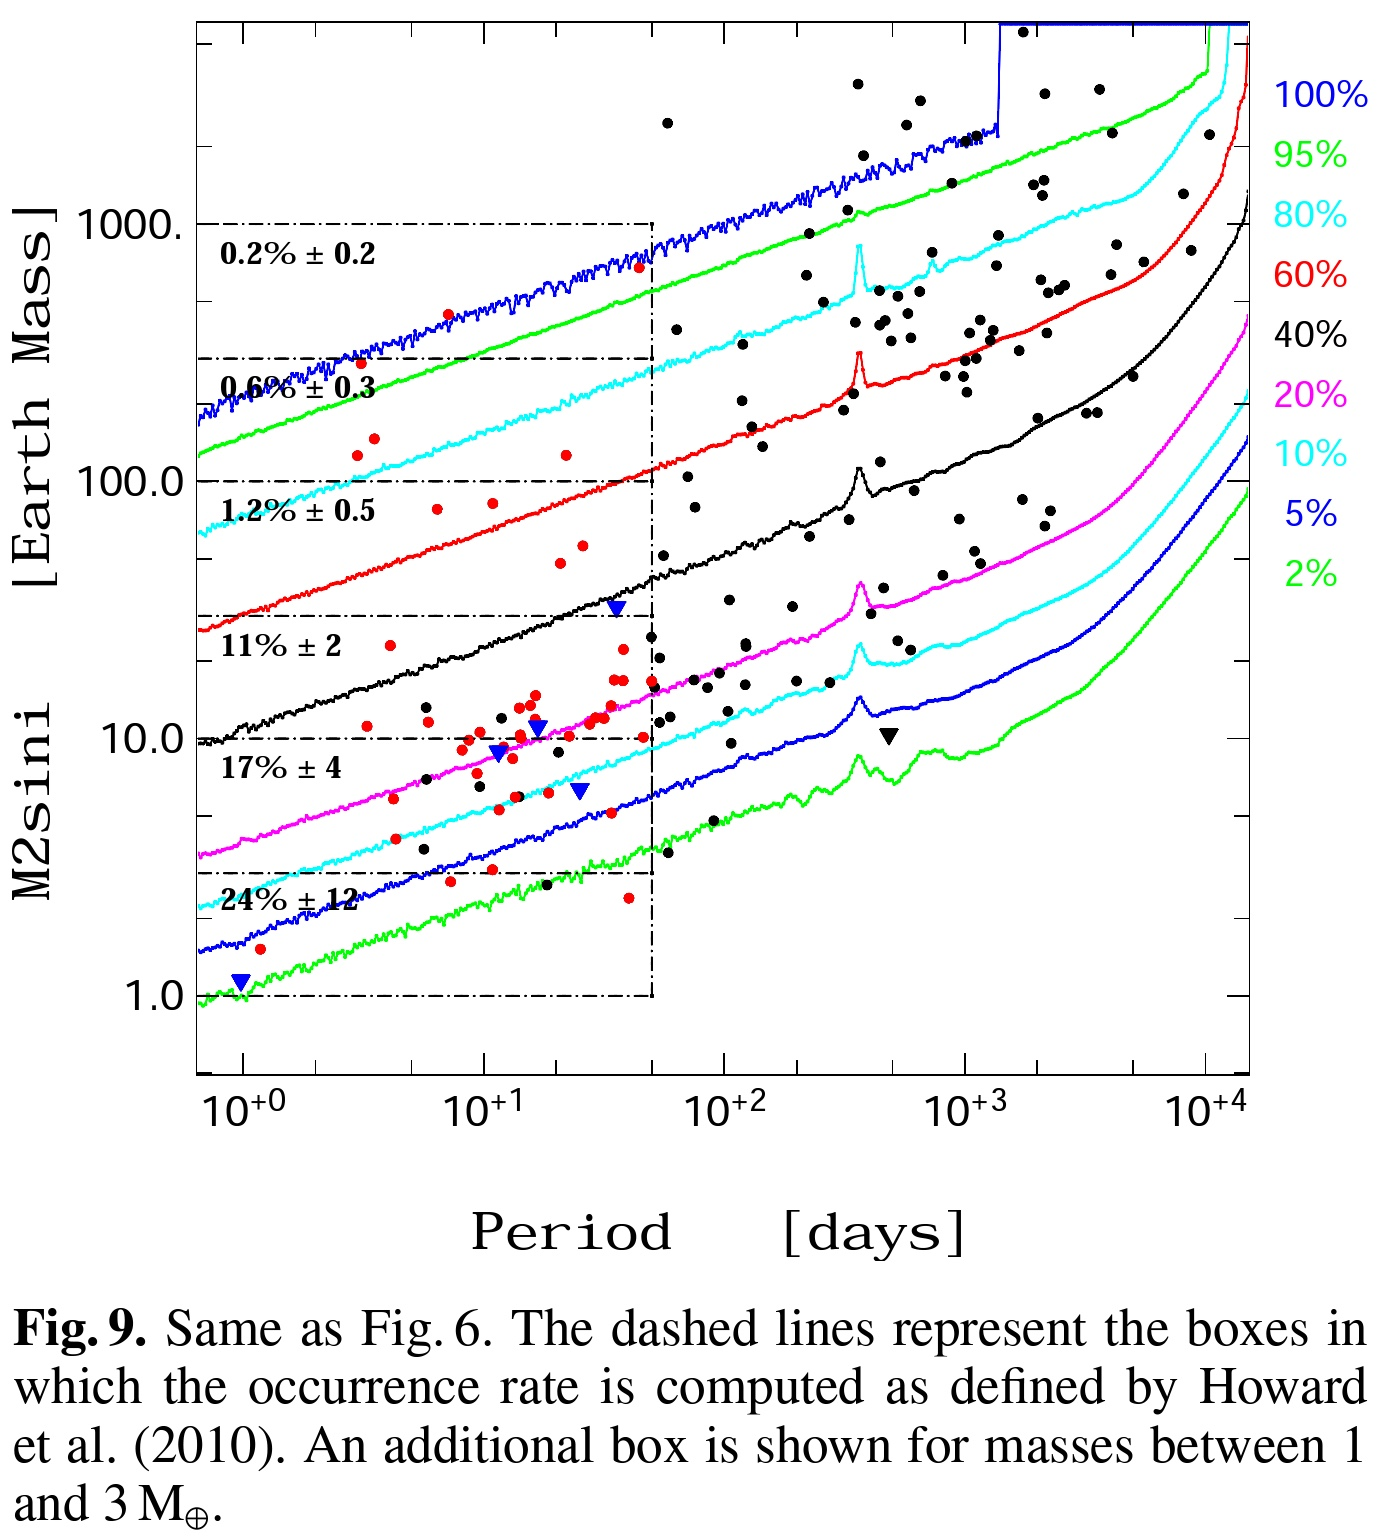
\includegraphics[trim={0cm 0cm 0 0},clip, keepaspectratio,height=0.45\textheight]{PMfreq-short}\label{fig:PMfreq-short}\end{figure}

\end{frame}

\begin{frame}{Distribuzione di massa: RV, Mayor 11}

\end{frame}

\begin{frame}{Distribuzione periodi: RV, Mayor 11}

\end{frame}

\begin{frame}{Caratteristiche orbitali: RV, Mayor 11}

\end{frame}

\begin{frame}{Sistemi multipli e metallicit\'a}

\end{frame}

\section{Properties of transit exoplanets}

\section{Orbital evolution}

\subsection{Hot Jupiters due to tidal circularization}

\begin{frame}{Planet-Planet scattering}
Scattering in eccentric close-in orbit. Tidal circularization: limit distance twice the Roche limit.
\end{frame}

\begin{wordonframe}{Tidal circularization}
During circularization angular momentum $\proto \sqrt{GMa(1-e^2)}$: for $e\approx1$: $a_f=a_i(1-e^2)\approx2a_{peri}$.

$R_p=0.462a_R(\frac{M_p}{M_*})\expy{\frac{1}{3}}$ 
\end{wordonframe}
